% article.tex
% Submission-ready article retargeted for Expert Systems with Applications (ESWA)
% Elsevier, single-column preprint/review format (line-numbered, double-spaced).
%
% Compile from the paper/ directory (twice for cross-references; no bibtex pass needed
% because the bibliography is a manual \thebibliography handled by natbib):
%   pdflatex -interaction=nonstopmode article.tex
%   pdflatex -interaction=nonstopmode article.tex

% ---------------------------------------------------------------------------
% DOCUMENT CLASS  (Elsevier elsarticle, single-column preprint with review
% line numbers; author-year forwarded to natbib via the class option, which is
% why natbib is NOT re-loaded below -- elsarticle already loads it.)
% ---------------------------------------------------------------------------
\documentclass[preprint,review,authoryear,12pt]{elsarticle}

% ---------------------------------------------------------------------------
% PACKAGES
% ---------------------------------------------------------------------------
\usepackage[T1]{fontenc}
\usepackage[utf8]{inputenc}
\usepackage[english]{babel}
\usepackage{microtype}

% Graphics (figures live in paper/figures/).
\usepackage{graphicx}
\graphicspath{{figures/}}

% Tables
\usepackage{booktabs}
\usepackage{tabularx}
\usepackage{array}

% Math
\usepackage{amsmath}
\usepackage{amssymb}

% Concept diagrams (self-contained, no external image files)
\usepackage{tikz}
\usetikzlibrary{arrows.meta,positioning,fit,backgrounds}

% Floats
\usepackage{float}

% Compact lists
\usepackage{enumitem}
\setlist{noitemsep, topsep=3pt}

% Hyperlinks (load late)
\usepackage{hyperref}

% ---------------------------------------------------------------------------
% DOCUMENT BEGIN
% ---------------------------------------------------------------------------
\begin{document}

\begin{frontmatter}

    \title{Reinforcement Learning vs.\ Rule-Based Policies for Dynamic Credit Threshold Control: A Simulation Study}

    \author[hse]{Evgeny Baulin\corref{cor1}\fnref{orcid1}}
    \ead{eabaulin@edu.hse.ru}
    \author[isp]{P.~P.~Lukianchenko\fnref{orcid2}}
    \ead{p.lukyanchenko@ispras.ru}

    \affiliation[hse]{organization={HSE University, Faculty of Computer Science},
        addressline={Bachelor's Programme ``Data Science and Business Analytics''},
        city={Moscow}, country={Russia}}
    \affiliation[isp]{organization={Trusted AI Research Center, Ivannikov Institute for System Programming of the RAS (ISP RAS)},
        city={Moscow}, country={Russia}}
    \cortext[cor1]{Corresponding author.}
    \fntext[orcid1]{ORCID: \href{https://orcid.org/0009-0004-9030-2893}{0009-0004-9030-2893}.}
    \fntext[orcid2]{ORCID: \href{https://orcid.org/0000-0002-1022-6041}{0000-0002-1022-6041}.}

    \begin{abstract}
        Portfolio-level credit acceptance thresholds are revised periodically in practice,
        which makes the decision sequential rather than one-shot. Each week the controller
        sets two acceptance thresholds, one for new clients and one for repeat clients, and
        then observes delayed repayment and default outcomes over subsequent weeks. We
        evaluate six deep reinforcement learning (RL) algorithms (DQN, Double-DQN, PPO, SAC,
        A3C, and A2C) against five rule-based baselines in a calibrated synthetic
        credit-portfolio simulator across six market scenarios and four observation-space
        sizes (12D, 20D, 30D, 50D). Data-driven weekly threshold control is one concrete way
        intelligent systems can improve business lending decisions, because adjusting
        thresholds to current portfolio and market signals can reduce realized default rates
        while protecting profit, and this study identifies when such automation pays off. The
        simulator is a calibrated proof-of-concept test bench, not a substitute for real
        banking data. Only observation dimensionality varies across the four conditions, with
        the simulator, reward, seeds, and evaluation protocol held fixed. We find that the
        constraint-aware weekly policy remains the best overall controller by cumulative
        reward (the primary ranking metric, with realized profit 3{,}802{,}547) and is
        statistically tied with the profit-oriented policy on realized profit, and RL still
        does not win the reward ranking in any scenario or dimension. Agents are trained for
            1{,}500 episodes per seed, a substantially larger budget than a short pilot run, and
        under this budget the best RL agent closes almost all of the profit gap to the
        leading baseline, from $-$9.4\% under a short 50-episode budget to between
        $-$0.5\% (12D, SAC) and $-$2.5\% (30D, DQN), and even wins raw profit in two of six
        scenarios at 12D (SAC). The strongest RL agent varies by dimension (SAC at 12D and
        50D, A2C at 20D, DQN at 30D), so no single algorithm dominates across the observation
        sizes. A controlled state-dimensionality comparison on the canonical DQN agent shows
        that 30D significantly outperforms both 12D and 50D on cumulative reward, and this is
        not only a reward effect: the best RL agent undercuts both profit-seeking baselines on
        default rate in five of six scenarios at 30D and 50D, versus one of six at 20D and
        zero of six at 12D, so the conditional risk-side advantage of richer state emerges
        specifically once the observation is rich enough. A delayed-evaluation check in the
        adverse-stress scenario shows near parity between DQN and the static-threshold
        baseline early in the horizon and a large, highly significant DQN advantage by the
        horizon midpoint, supporting a ``locally tied, globally better'' pattern. Episode-static
        behavior, in which a controller fixes a threshold pair at the start of an episode and
        barely adjusts it, is no longer universal: it is specific to the DQN family at
        12--30D, while SAC and the actor-critic agents adjust thresholds within the episode at
        every dimension. We conclude that, given a sufficient training budget, RL becomes
        highly competitive with well-designed rule-based weekly threshold search, though the
        strongest rule-based policies still win the primary reward ranking in every scenario
        and dimension tested.
    \end{abstract}

    \begin{keyword}
        Reinforcement Learning \sep Credit Scoring \sep Threshold Control \sep
        Markov Decision Process \sep Delayed Rewards \sep Portfolio Simulation \sep
        Rule-Based Policies \sep State Dimensionality
    \end{keyword}

\end{frontmatter}

% ===========================================================================
\section{Introduction}
% ===========================================================================

A credit manager who holds a single static acceptance threshold loses money as the
portfolio composition, the capital usage, and the market conditions drift between
decisions. In practice, banks and consumer-lending institutions revise acceptance
thresholds periodically rather than once. The fraction of applicants to approve this
week depends on the current portfolio composition, outstanding capital commitments,
rolling default rates, and market conditions that evolve between decisions. The weekly
acceptance decision is therefore a recurring control problem, not a one-shot cut-off.
Much of the academic literature has instead treated threshold selection as a one-shot
classification problem, estimating a default probability, choosing a cut-off, and
evaluating by AUC or Gini, which ignores the sequential nature of actual threshold
management \citep{thomas2017, lessmann2015}. That gap between static cut-off
optimisation and dynamic portfolio management motivates the present study.

We build and evaluate an intelligent decision-support module for weekly threshold
control, and we compare learned (RL) controllers against strong rule-based expert
policies. Data-driven weekly threshold control is one concrete way artificial
intelligence can improve business lending decisions. By adjusting acceptance
thresholds to current portfolio and market signals, it can reduce realized defaults
while protecting profit, and the present study identifies the conditions under which
such automation pays off. Reinforcement learning provides a natural framework for
decisions with delayed consequences \citep{arulkumaran2017}. An RL agent observes the
state of the portfolio, selects a pair of weekly thresholds, and receives a reward
signal that reflects realized portfolio cash flows rather than immediate cohort
expectations. The delayed-outcome setting is central: a loan accepted at week $t$ may
not default or repay until week $t + \Delta$, so the correct evaluation object is the
full portfolio trajectory, not the immediately observable cohort.
\citet{herasymovych2019} showed that a DQN agent can learn to adjust a single
acceptance threshold in a simulated credit environment with delayed outcomes,
establishing the structural ideas on which this study builds.

\paragraph{Calibration disclaimer}
All experiments in this paper use a synthetic simulator calibrated to published retail
lending statistics (Bank of Russia supervisory data and ECB SSM loan loss reports) as
a controlled proof-of-concept test bench. Synthetic simulation is standard practice in
RL-based credit research because real loan-level panels with weekly cohort granularity
and observable repayment and default events are not publicly available
\citep{herasymovych2019, lessmann2015}. The simulator provides full control over market
regime, segment composition, and shock timing, which makes the multi-scenario
robustness evaluation possible. Results should be interpreted as evidence about
algorithmic behaviour under these controlled conditions, not as forecasts for any
specific production portfolio.

The paper extends the framework of \citet{herasymovych2019} with four contributions:
(i) split weekly thresholds for new and repeat client segments, (ii) a controlled
state-dimensionality experiment comparing 12D, 20D, 30D, and 50D observation sizes
under a fixed protocol, (iii) five economically meaningful rule-based baselines as the
comparison standard, and (iv) statistical hypothesis tests on paired run-level data.
The central research question is:
\begin{quote}
    \emph{Under which conditions does reinforcement learning provide a robust improvement
        over rule-based threshold policies in a delayed-outcome credit-scoring environment?}
\end{quote}
The data give a conditional answer. Strong rule-based weekly search wins every scenario
and dimension by the primary reward ranking, and with a training budget large enough for
the RL agents to approach convergence (1{,}500 episodes per seed) the best RL agent closes
almost all of the profit gap to the leading baseline and even wins raw profit in two of
six scenarios at 12D. Richer-state RL agents also produce lower portfolio default rates
than the profit-seeking baselines in a majority of scenarios once the state is rich enough
(five of six scenarios at 30D and 50D, versus one of six at 20D and zero of six at 12D),
while the risk-aware weekly policy stays the single lowest-default controller overall.
This points to a conditional risk-side advantage that becomes visible once the profit
ranking is supplemented by credit-quality metrics, and that itself depends on observation
dimensionality.

% ===========================================================================
\section{Related Work}
% ===========================================================================

Traditional credit scoring estimates default probability at the application level and
selects a cut-off that balances interest income against expected loss
\citep{thomas2017, hand1997, siddiqi2006}. Benchmarking studies have shown that
classifier rankings depend on the dataset and the evaluation protocol, and that
logistic regression and gradient-boosted trees are difficult to outperform with more
complex classifiers \citep{lessmann2015, baesens2003}. The same conclusion recurs in
more recent work: \citet{gunnarsson2021} find that deep neural networks do not reliably
beat gradient boosting on standard credit datasets, and reviews of consumer credit risk
assessment reach a similar verdict on where modelling effort actually pays off
\citep{zhangyu2023}. Application-oriented research has therefore shifted from raw
classifier accuracy toward feature enhancement and ensembling \citep{yang2024}
and toward explainability for credit decisions \citep{nallakaruppan2024}, reflecting the
practical priorities of intelligent lending systems.

These advances still treat the accept/reject cut-off as a static one-shot tuning step.
A second line of work reframes threshold choice as a cost-sensitive economic decision
rather than a classification metric \citep{baesens2003}, and \citet{bellotti2009} note
that under Basel\,II/III capital adequacy requirements the threshold affects outstanding
exposure, realized losses, and regulatory capital in ways that make static cut-off
selection insufficient once market conditions or portfolio composition drift over time.
Once the decision is recognised as recurring and state-dependent, it becomes a
sequential control problem, which is the natural domain of reinforcement learning.

Reinforcement learning addresses problems with delayed consequences through the Markov
Decision Process (MDP) framework \citep{dayan2008, arulkumaran2017}. The deep RL
algorithms used in this study illustrate the main design axes. DQN couples Q-learning
with experience replay for off-policy sample efficiency on discrete action spaces,
Double-DQN reduces the overestimation bias of vanilla DQN \citep{van2016ddqn}, PPO is an
on-policy policy-gradient method with stable updates \citep{schulman2017ppo}, SAC is an
off-policy maximum-entropy actor-critic \citep{haarnoja2018sac}, and A3C and A2C are
asynchronous and synchronous actor-critic variants. A broad survey of these methods
appears in \citet{arulkumaran2017}. In this study A2C, PPO, and SAC use the
Stable-Baselines3 implementations \citep{stable_baselines3}, while DQN, Double-DQN, and
A3C use matched custom PyTorch implementations.

Applying RL to credit control is more recent and still thin. \citet{herasymovych2019}
optimise the acceptance threshold of a credit-scoring model with RL in a simulated
environment with delayed outcomes, and \citet{kiatsupaibul2024} survey reinforcement
learning for credit scoring and underwriting and note how few controlled comparisons
against strong rule-based policies exist. The direct precursor \citep{herasymovych2019}
compared a DQN agent against a single static threshold in one scenario using a shared,
non-split threshold. No prior work has simultaneously evaluated split thresholds for
distinct borrower segments, a controlled observation-dimensionality comparison, strong
economically motivated rule-based baselines, and six market scenarios with statistical
testing. That combination is the gap this paper fills, and it motivates the three
hypotheses stated in Section~\ref{sec:hypotheses}.

% ===========================================================================
\section{Problem Formulation and Methodology}
% ===========================================================================

\subsection{MDP Formulation}

We model the weekly threshold-control problem as a discrete-time MDP
$(\mathcal{S}, \mathcal{A}, \mathcal{P}, r, \gamma)$. The \textbf{state}
$s_t \in \mathbb{R}^d$ ($d \in \{12, 20, 30, 50\}$) is a portfolio summary vector
observed at the beginning of interactive week $t$. It includes approval rates, default
rates, realized profit and NPV, capital usage, outstanding exposure, segment shares,
and, at higher dimensionalities, lagged and rolling history. The \textbf{action} is a
pair of acceptance thresholds
$a_t = (\tau^{\text{new}}_t, \tau^{\text{repeat}}_t) \in \{35, 40, \ldots, 85\}^2$:
applications from new (repeat) clients with credit score above $\tau^{\text{new}}_t$
($\tau^{\text{repeat}}_t$) are accepted. This yields $11 \times 11 = 121$ joint actions
per week. The \textbf{reward} is described in Section~\ref{sec:reward}. The discount
factor is $\gamma = 0.98$.

Figure~\ref{fig:mdp-loop} shows the weekly decision loop as a Markov decision process.
The figure makes explicit that each weekly action is scored only through delayed cash
flows, so the controller must account for outcomes that arrive several weeks after the
threshold is set.

\begin{figure}[t]
    \centering
    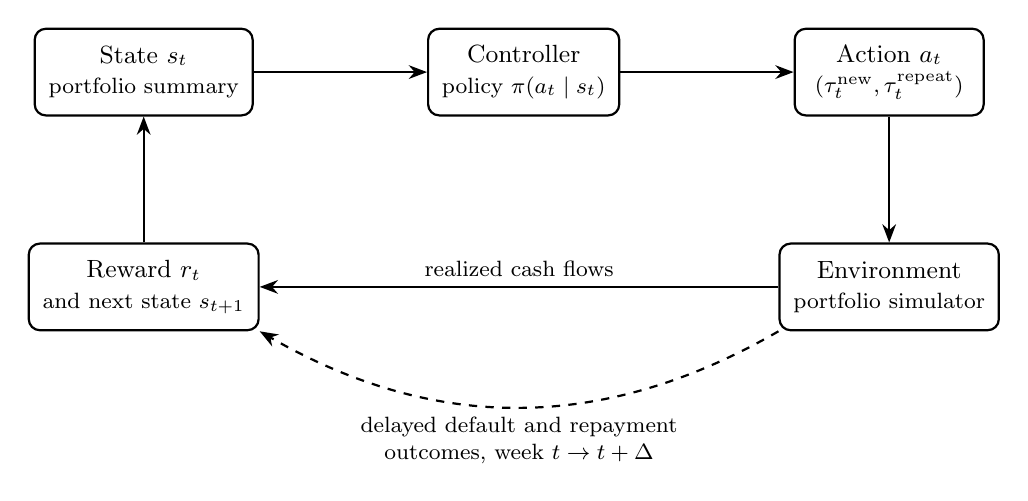
\begin{tikzpicture}[>=Stealth, thick, font=\small,
            box/.style={draw, rounded corners, align=center, inner sep=5pt,
                    minimum height=11mm, minimum width=24mm}]
        \node[box] (state) {State $s_t$\\ {\footnotesize portfolio summary}};
        \node[box, right=22mm of state] (policy) {Controller\\ {\footnotesize policy $\pi(a_t\mid s_t)$}};
        \node[box, right=22mm of policy] (action) {Action $a_t$\\ {\footnotesize $(\tau^{\mathrm{new}}_t,\tau^{\mathrm{repeat}}_t)$}};
        \node[box, below=16mm of action] (env) {Environment\\ {\footnotesize portfolio simulator}};
        \node[box, below=16mm of state] (reward) {Reward $r_t$\\ {\footnotesize and next state $s_{t+1}$}};
        \draw[->] (state) -- (policy);
        \draw[->] (policy) -- (action);
        \draw[->] (action) -- (env);
        \draw[->] (env) -- node[above, font=\footnotesize]{realized cash flows} (reward);
        \draw[->] (reward) -- (state);
        \draw[->, dashed] (env.south west) to[out=210, in=330]
        node[below, font=\footnotesize, align=center]
        {delayed default and repayment\\ outcomes, week $t \to t+\Delta$} (reward.south east);
    \end{tikzpicture}
    \caption{Weekly threshold control as a Markov decision process. The dashed arrow marks
        the delayed default and repayment outcomes that link an action taken at week $t$ to
        rewards realized at later weeks $t+\Delta$.}
    \label{fig:mdp-loop}
\end{figure}

\subsection{Simulation Environment}

Each episode consists of three phases. (1) An \textbf{8-week warm-up} pre-fills the loan
book using default thresholds before the controller begins acting. (2) During the
\textbf{52-week interactive horizon} the controller sets weekly thresholds. The simulator
generates applications from Gaussian credit scores clipped to $[0,100]$ for new and repeat segments,
applies a logistic default-probability mapping, accepts loans above the threshold, and
schedules repayment, default, and recovery events in a forward event queue.
(3) \textbf{Terminal settlement} resolves all pending cash flows at episode end so that
loans originated near the horizon are not mechanically penalized. Default probabilities
are calibrated to target 4--6\% in the base scenario and 9--14\% under adverse stress,
consistent with published retail lending statistics.

Figure~\ref{fig:episode} shows the three-phase episode structure and the within-week
loan lifecycle. The figure shows that outcomes from accepted loans are pushed into a
forward event queue, so repayments, defaults, and recoveries feed back into later weeks
rather than into the week of origination.

\begin{figure}[t]
    \centering
    \resizebox{\linewidth}{!}{%
        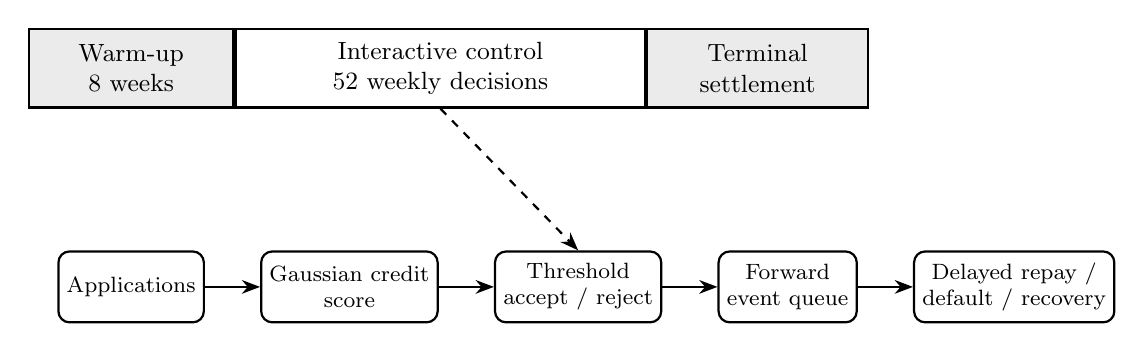
\begin{tikzpicture}[>=Stealth, thick, font=\small,
                phase/.style={draw, minimum height=10mm, align=center, inner sep=4pt},
                lstep/.style={draw, rounded corners, align=center, font=\footnotesize,
                        inner sep=3pt, minimum height=9mm}]
            \node[phase, fill=black!8, minimum width=26mm] (warm) {Warm-up\\ 8 weeks};
            \node[phase, minimum width=52mm, right=0mm of warm] (inter) {Interactive control\\ 52 weekly decisions};
            \node[phase, fill=black!8, minimum width=28mm, right=0mm of inter] (term) {Terminal\\ settlement};
            \node[lstep, below=18mm of warm] (apps) {Applications};
            \node[lstep, right=7mm of apps] (score) {Gaussian credit\\ score};
            \node[lstep, right=7mm of score] (thr) {Threshold\\ accept / reject};
            \node[lstep, right=7mm of thr] (queue) {Forward\\ event queue};
            \node[lstep, right=7mm of queue] (out) {Delayed repay /\\ default / recovery};
            \draw[->] (apps) -- (score);
            \draw[->] (score) -- (thr);
            \draw[->] (thr) -- (queue);
            \draw[->] (queue) -- (out);
            \draw[->, dashed] (inter.south) -- (thr.north);
        \end{tikzpicture}}
    \caption{Episode structure and loan lifecycle. The top row is the episode timeline
        (8-week warm-up, 52-week interactive weekly control, terminal settlement), and the
        bottom row is the within-week sequence from application to delayed outcome.}
    \label{fig:episode}
\end{figure}

In Table~\ref{tab:scenarios}, the six evaluation scenarios and their primary stress
mechanism are listed. The scenarios probe distinct portfolio-management weaknesses, so a
controller that performs well across all of them is robust rather than tuned to a single
regime.

\begin{table}[t]
    \centering
    \small
    \caption{The six evaluation scenarios and their primary stress mechanism.}
    \label{tab:scenarios}
    \begin{tabularx}{0.96\linewidth}{>{\ttfamily}p{0.26\textwidth}X}
        \toprule
        Scenario                & Stress mechanism                                               \\
        \midrule
        base\_market            & Stable, the cleanest test of policy signal exploitation        \\
        drift                   & Gradual new-client score deterioration and rising defaults     \\
        adverse\_stress         & Abrupt shock: higher defaults, larger loans, capital pressure  \\
        class\_imbalance\_shift & Growing share of weaker new applicants, tests composition risk \\
        noise                   & Stable mean with noisy weekly volumes and measurements         \\
        split\_policy\_dynamics & New clients deteriorate while repeat clients improve           \\
        \bottomrule
    \end{tabularx}
\end{table}

\subsection{Agents and Baselines}

\textbf{RL agents.}\;
All six agents use a shared two-layer MLP ($2 \times 128$ hidden units) and a fixed set
of hyperparameters held identical across the four state sizes (\ref{app:hyperparams}).
A2C, PPO, and SAC use Stable-Baselines3, while DQN, Double-DQN, and A3C use matched
custom PyTorch implementations. No per-dimension hyperparameter search is performed, so
any performance difference across dimensions is attributable to the observation vector
rather than to the training recipe.

\textbf{Rule-based baselines} span five management styles. The static-threshold
baseline (\texttt{static\_threshold}) applies one fixed shared threshold. The
split-static baseline (\texttt{split\_policy\_static}) maintains separate fixed defaults
per segment. The profit-oriented policy (\texttt{profit\_oriented}) performs a weekly
grid search maximising current-cohort expected profit without penalty terms. The
risk-aware weekly policy (\texttt{risk\_aware\_weekly}) adjusts thresholds reactively to
rolling default pressure and capital signals. The constraint-aware weekly policy
(\texttt{constraint\_aware\_weekly}) runs a penalty-weighted weekly grid search that
explicitly internalises default-rate, approval-rate, capital-usage, and volatility
violations.

\subsection{Reward Function}
\label{sec:reward}

With delayed reward enabled, the shaped weekly reward is:
\begin{equation}
    \label{eq:reward}
    \begin{aligned}
        r_t ={} & \;
        w_p\,\Pi^{\text{realized}}_t
        + w_n\,\mathrm{NPV}^{\text{realized}}_t
        - w_s\,\hat{d}_t \cdot 100                                                                   \\
                & - \lambda_d\!\left[\max\!\bigl(0,\,\bar{d}_t - 0.12\bigr)\right]^{\!2}\!\cdot 1000
        - \lambda_a\left|\alpha_t - 0.42\right|\cdot 1000                                            \\
                & - \lambda_c\!\left[\max\!\bigl(0,\,c_t - 0.82\bigr)\right]^{\!2}\!\cdot 1000
        - \lambda_v\max\!\!\left(0,\,\frac{\sigma_{\Pi,t}-8500}{8500}\right)\!\cdot 1000,
    \end{aligned}
\end{equation}
where $\Pi^{\text{realized}}_t$ and $\mathrm{NPV}^{\text{realized}}_t$ are realized
weekly profit and NPV (not current-cohort expectations), $\hat{d}_t$ is the expected
default rate of the current cohort, $\bar{d}_t$ is the rolling realized default rate,
$\alpha_t$ is the weekly approval rate, $c_t$ is the projected capital usage ratio, and
$\sigma_{\Pi,t}$ is realized profit volatility. The four constants are calibration
targets: the default-rate cap ($0.12$), the target approval rate ($0.42$), the
capital-usage cap ($0.82$), and the profit-volatility scale ($8500$). Active weights:
$w_p{=}1.0$, $w_n{=}0.25$, $w_s{=}0.35$, $\lambda_d{=}9.0$, $\lambda_a{=}2.0$,
$\lambda_c{=}3.5$, $\lambda_v{=}1.4$.

The reward is multi-objective by design. Rankings by cumulative reward need not coincide
with rankings by raw profit, because the reward encodes portfolio risk constraints
rather than profit alone. Throughout this paper, ``realized profit'' is computed from
realized interactive weekly profits plus terminal settlement, that is, realized final
portfolio profit rather than a current-cohort expectation.

% ===========================================================================
\section{Experimental Design}
% ===========================================================================

The experiment is fully controlled: \emph{only} observation dimensionality varies across
the four runs. Everything else (the simulator, the reward, the eight random seeds, the
    1{,}500 training episodes per seed, the evaluation protocol, the scenarios, the threshold
grid, and the controller set) is held fixed. Each of the six agents is trained once per
state dimension per seed (6~agents~$\times$~4~dimensions~$\times$~8~seeds~$=192$ training
runs, each running the full 1{,}500-episode budget with the training scenario drawn from a
pool of all six market scenarios), and evaluated over
6~scenarios~$\times$~8~seeds~$\times$~12~evaluation~runs~$=576$ evaluation runs per
controller per dimension. A validity layer programmatically verifies that the first 12
observation features are bit-for-bit identical across all four state sizes on a common
reset and three fixed-action transitions.

In Table~\ref{tab:state-layers}, the cumulative composition of the four observation
layers is shown, where each layer adds features that a portfolio manager would
realistically observe at weekly decision time with no access to future outcomes. Because
each layer is a superset of the previous one, observation dimensionality is the only
factor that changes across the four conditions.

\begin{table}[t]
    \centering
    \small
    \caption{Cumulative observation layers. The first 12 features are invariant across all
        configurations and are verified programmatically before each experiment.}
    \label{tab:state-layers}
    \begin{tabularx}{0.96\linewidth}{>{\centering\arraybackslash}p{0.06\textwidth}
            >{\raggedright\arraybackslash}X}
        \toprule
        Size & Added information                                                             \\
        \midrule
        12D  & Compact dashboard: week progress, overall/segment approval rates,
        rolling realized default rate, expected default rate, realized profit, profit
        volatility, projected capital usage, outstanding ratio, both threshold levels.       \\
        20D  & 12D~+ current economic context: repeat segment share, expected profit/NPV per
        application, realized NPV, weekly reward, threshold gap, capital headroom,
        realized-vs-expected default gap.                                                    \\
        30D  & 20D~+ lagged/rolling memory: second-lag approval/default/profit/capital,
        four-week rolling means and std of approval, default, and profit, lagged
        threshold changes.                                                                   \\
        50D  & 30D~+ segment-specific signals and stability descriptors: segment approval/
        default/profit indicators, accepted-share ratios, rolling reward moments,
        cumulative reward/profit to date, capital-usage volatility, outstanding-ratio
        changes, threshold-gap history, application-volume ratio.                            \\
        \bottomrule
    \end{tabularx}
\end{table}

\subsection{Hypotheses}
\label{sec:hypotheses}

The three hypotheses follow from the research gap and from the literature reviewed in
Section~2, and each is tested on paired run-level data in Section~\ref{sec:stat-tests}.
The first hypothesis concerns state representation. Because feature enhancement and
richer inputs are repeatedly reported to help credit models up to a point
\citep{yang2024}, we expect added observation features to improve the RL
frontier but only over an intermediate range. The second hypothesis concerns the RL
advantage. The credit-scoring benchmarking literature repeatedly finds that more complex
models do not reliably dominate simpler ones \citep{lessmann2015, gunnarsson2021}, and
the direct precursor compared RL against only a single static baseline
\citep{herasymovych2019, kiatsupaibul2024}, so we expect the universal-dominance claim to
fail against strong rule-based policies. The third hypothesis concerns delayed
evaluation. Because outcomes are delayed and terminal settlement is applied, as in the
delayed-reward credit-control setting of \citet{herasymovych2019}, early-period
performance may misrepresent final portfolio quality.

\begin{description}[leftmargin=2.2em,style=nextline]
    \item[H1 (State representation).] Richer state representations improve the best RL
          frontier from 12D to 30D, while the move from 30D to 50D does not necessarily
          create additional improvement.
    \item[H2 (RL vs.\ rule-based).] RL improves over rule-based policies only in some
          scenarios and metrics, and the universal claim that RL robustly dominates strong
          rule-based baselines is expected to be \emph{rejected}.
    \item[H3 (Delayed evaluation).] Early-period performance is an unreliable proxy for
          final realized portfolio quality when outcomes are delayed and terminal
          settlement is applied. The ``locally worse, globally better'' pattern is expected
          to hold.
\end{description}

% ===========================================================================
\section{Results}
% ===========================================================================

\subsection{Best Overall and Best RL Controller by Dimension}

In Table~\ref{tab:best-by-dim}, the strongest controller is reported when baselines and
RL agents are pooled under the repository's official ranking rule (highest cumulative
reward, then highest profit, then lowest default rate), together with the strongest RL
controller in each dimension (full-profile run, 8 seeds $\times$ 1{,}500 episodes per
seed, with data and configuration in the public repository). Unlike under the short
50-episode budget, the best RL agent is not the same algorithm at every dimension: SAC
leads at 12D and 50D, A2C at 20D, and DQN at 30D. The best RL profit still peaks at 12D
and dips at 30D before partially recovering at 50D, but the gap to the leading baseline is
now small at every dimension.

\begin{table}[t]
    \centering
    \small
    \caption{Best overall controller and best RL controller by state dimension
        (full-profile run, 1{,}500 training episodes per seed). The baseline line is flat
        because the leading baseline does not depend on the RL observation vector. ``Profit''
        is realized final portfolio profit (Section~\ref{sec:reward}); ``Reward'' is
        cumulative shaped reward.}
    \label{tab:best-by-dim}
    \setlength{\tabcolsep}{4pt}
    \begin{tabular}{c l l r r r}
        \toprule
        Dim & Controller              & Type     & Profit        & Reward        & Default rate \\
        \midrule
        \multicolumn{6}{l}{\textit{Best overall (pooled, by cumulative reward)}}                \\
        12  & Constraint-aware weekly & baseline & 3{,}802{,}547 & 3{,}666{,}052 & 0.0760       \\
        20  & Constraint-aware weekly & baseline & 3{,}802{,}547 & 3{,}666{,}052 & 0.0760       \\
        30  & Constraint-aware weekly & baseline & 3{,}802{,}547 & 3{,}666{,}052 & 0.0760       \\
        50  & Constraint-aware weekly & baseline & 3{,}802{,}547 & 3{,}666{,}052 & 0.0760       \\
        \midrule
        \multicolumn{6}{l}{\textit{Best RL agent}}                                              \\
        12  & SAC                     & RL       & 3{,}785{,}010 & 3{,}631{,}406 & 0.0768       \\
        20  & A2C                     & RL       & 3{,}761{,}562 & 3{,}624{,}570 & 0.0768       \\
        30  & DQN                     & RL       & 3{,}706{,}594 & 3{,}633{,}945 & 0.0749       \\
        50  & SAC                     & RL       & 3{,}724{,}499 & 3{,}605{,}339 & 0.0762       \\
        \bottomrule
    \end{tabular}
\end{table}

By cumulative reward, the primary ranking metric, the constraint-aware weekly policy is
the best overall controller in every dimension (reward 3{,}666{,}052). On raw realized
profit it is statistically tied with the profit-oriented policy, which is marginally
higher (3{,}803{,}168 vs.\ 3{,}802{,}547). The two differ by less than $0.02\%$ and the
difference is not economically meaningful. The flat baseline row confirms that the
experiment isolates the effect of observation size on RL quality, because the leading
rule-based policy is independent of the RL state vector by construction. With the
    1{,}500-episode budget, the profit gap between the best RL agent and the best overall
controller shrinks to $-$17{,}537 ($-$0.46\%) at 12D, $-$40{,}985 ($-$1.08\%) at 20D,
$-$95{,}953 ($-$2.52\%) at 30D, and $-$78{,}049 ($-$2.05\%) at 50D, and the corresponding
reward gaps are $-$34{,}646 ($-$0.95\%), $-$41{,}482 ($-$1.13\%), $-$32{,}108
($-$0.88\%), and $-$60{,}713 ($-$1.66\%). Every gap is under 2.6\% of the baseline value,
compared with $-$9.4\% for the best RL agent's 12D peak under the short 50-episode
budget, so the dominant effect of the larger training budget is to close most of the
RL-to-baseline gap rather than to change which controller wins. Default rate for the best
RL agent is 7.68\% at 12D, 7.68\% at 20D, 7.49\% at 30D, and 7.62\% at 50D, again lowest
at 30D, which foreshadows the risk-side pattern developed in
Section~\ref{sec:scenario-winners}.

Figure~\ref{fig:saturation} shows the same comparison as a function of observation
dimensionality. The figure shows that the best RL agent's profit is close to the leading
baseline at every dimension, with a shallow dip at 30D, while on default rate the best RL
agent moves from above the baseline line at 12D and 20D to below it at 30D and 50D --
richer state does not change who wins the reward ranking, but it does change whether RL's
default rate is competitive with the profit-seeking baselines.

\begin{figure}[t]
    \centering
    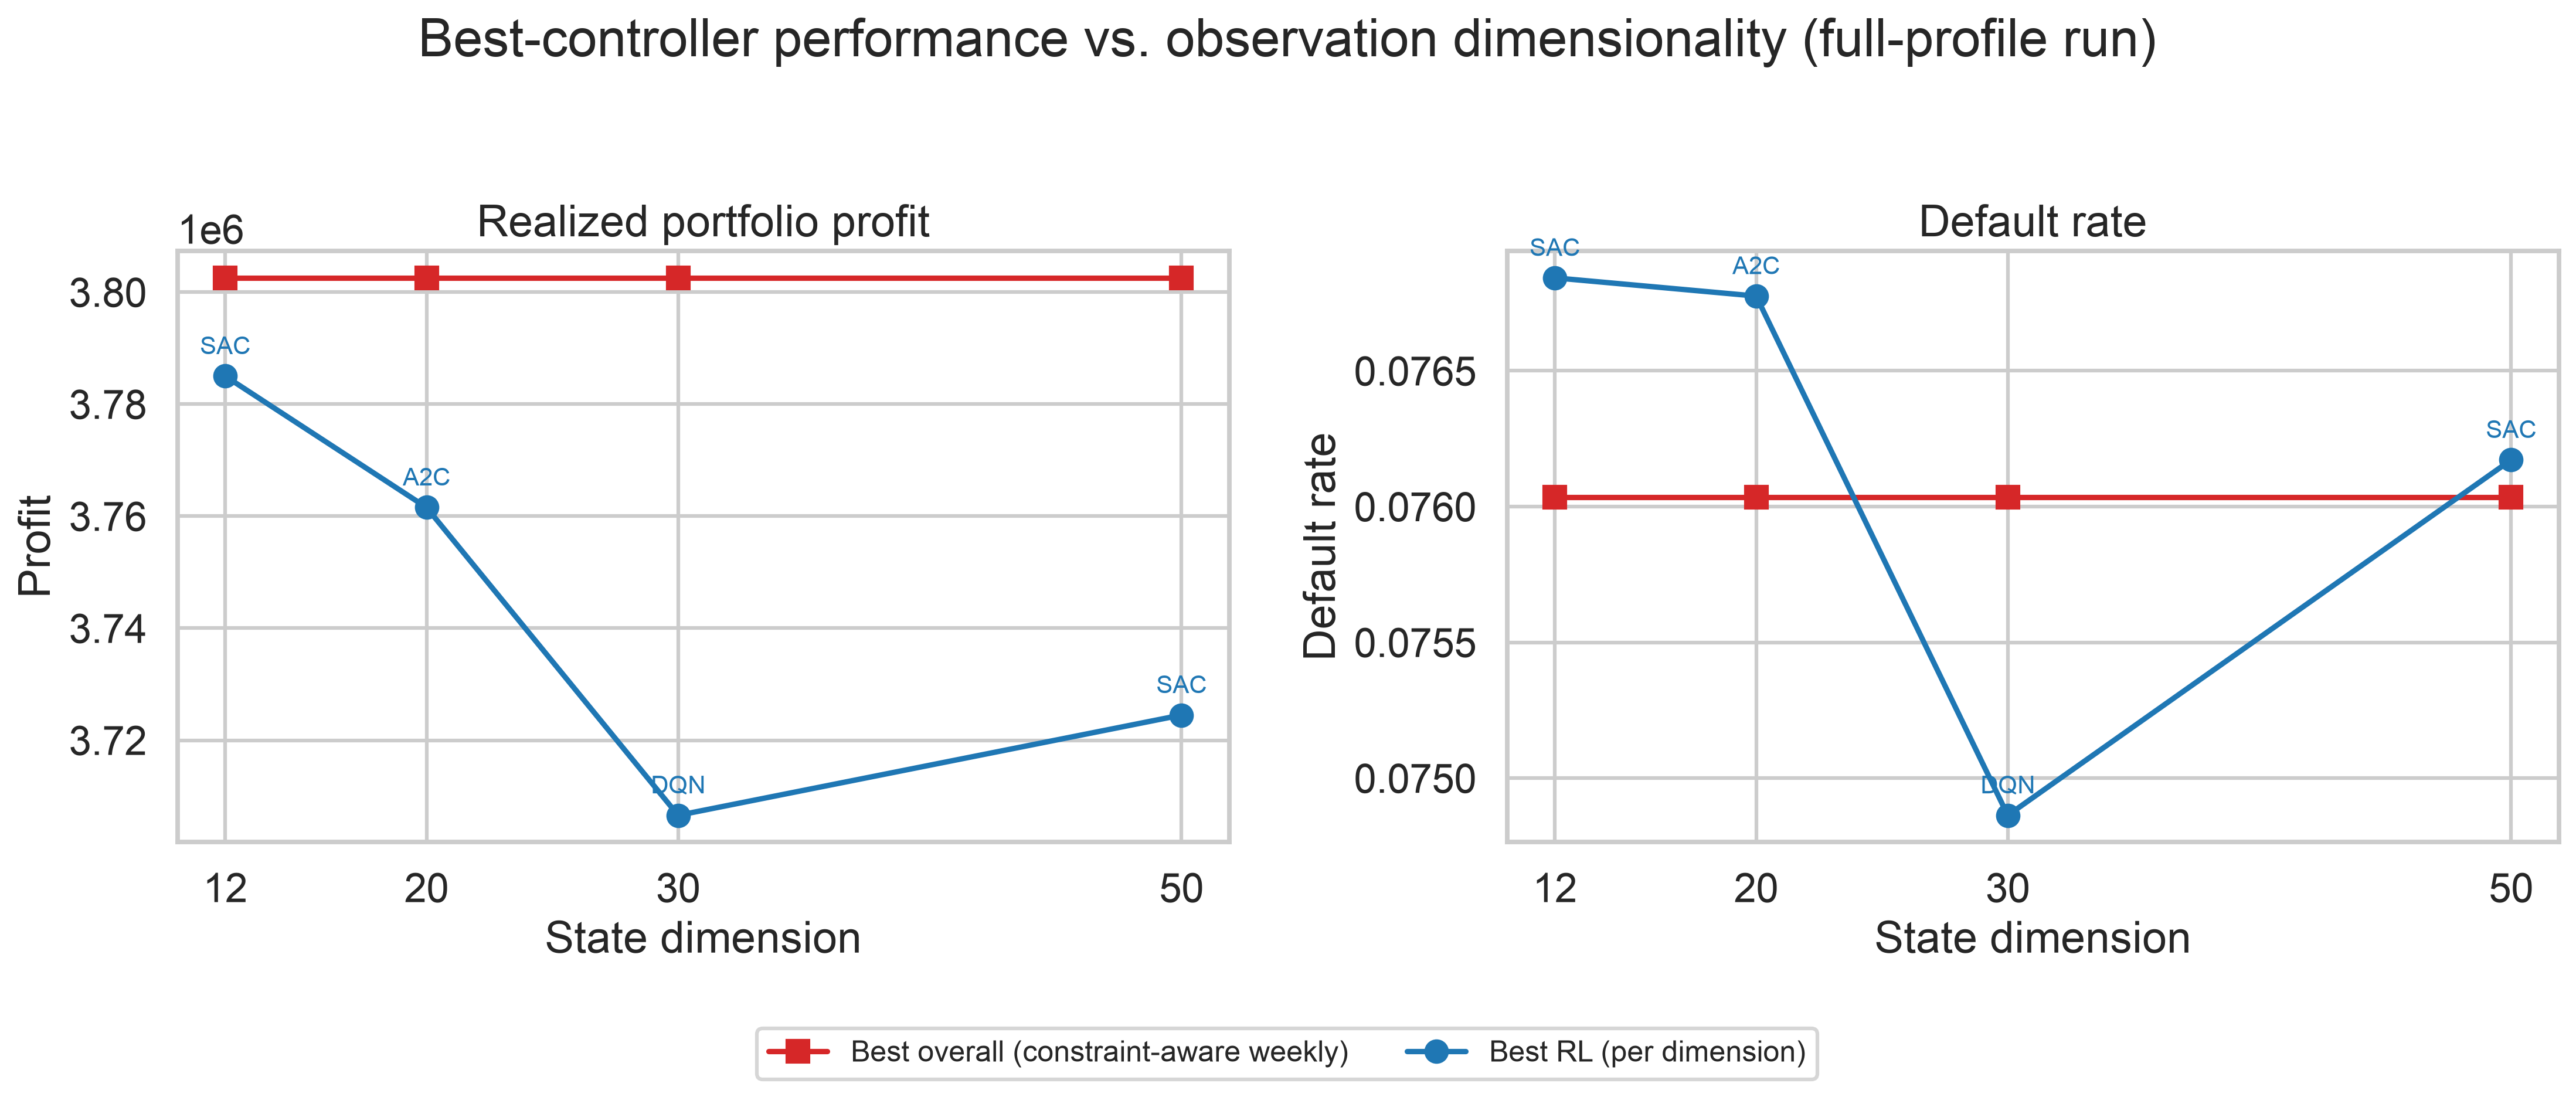
\includegraphics[width=0.98\linewidth]{dimensionality_saturation.png}
    \caption{Best-controller performance versus observation dimensionality (full-profile
        run, 8 seeds, 1{,}500 training episodes per seed). \textit{Left}: realized portfolio
        profit. \textit{Right}: default rate. The best overall controller (the
        constraint-aware weekly policy) is independent of the RL state vector and is
        therefore flat across dimensions, while the best RL agent (labelled per point: SAC
        at 12D and 50D, A2C at 20D, DQN at 30D) sits close to the baseline on profit at every
        dimension and crosses below the baseline on default rate at 30D and 50D.}
    \label{fig:saturation}
\end{figure}

\subsection{Agent Comparison}
\label{sec:agent-comparison}

In Table~\ref{tab:agent-summary}, the mean performance of each agent across all four
dimensions is summarised alongside the three principal rule-based baselines (full-profile
run, 1{,}500 training episodes per seed). With this larger budget the RL ranking is very
different from a short-budget run: SAC leads all RL agents on mean profit and comes
within 2.7\% of the best baseline's mean profit, PPO remains the weakest and most
degenerate agent, and the DQN family is no longer the strongest RL agent on average even
though it supplies the canonical reference agent for the hypothesis tests in
Section~\ref{sec:stat-tests}.

\begin{table}[t]
    \centering
    \small
    \caption{Agent and baseline summary (mean across all four dimensions, full-profile
        run, 1{,}500 training episodes per seed). ``Approval'' denotes mean weekly approval
        rate. Baseline rows do not depend on state dimension, so their per-dimension values
        are identical and the mean equals any single dimension's value.}
    \label{tab:agent-summary}
    \begin{tabular}{l l r r r}
        \toprule
        Controller              & Type     & Mean profit   & Default rate & Approval \\
        \midrule
        Profit-oriented         & baseline & 3{,}803{,}168 & 7.61\%       & 94.91\%  \\
        Constraint-aware weekly & baseline & 3{,}802{,}547 & 7.60\%       & 94.84\%  \\
        Static-threshold        & baseline & 3{,}083{,}370 & 6.62\%       & 69.99\%  \\
        \midrule
        SAC                     & RL       & 3{,}700{,}732 & 7.64\%       & 92.58\%  \\
        A2C                     & RL       & 3{,}607{,}319 & 7.59\%       & 90.12\%  \\
        A3C                     & RL       & 3{,}472{,}312 & 7.17\%       & 83.28\%  \\
        DQN                     & RL       & 3{,}393{,}809 & 7.36\%       & 82.68\%  \\
        Double-DQN              & RL       & 3{,}390{,}977 & 7.24\%       & 81.97\%  \\
        PPO                     & RL       & 2{,}617{,}957 & 6.21\%       & 57.16\%  \\
        \bottomrule
    \end{tabular}
\end{table}

SAC leads all RL agents on mean profit (3{,}700{,}732), only 2.7\% below the leading
baseline's mean profit (3{,}803{,}168), a striking change from the $-$9.4\% gap of the
best RL agent under a short 50-episode budget. A2C is a close second (3{,}607{,}319).
DQN and Double-DQN, the two off-policy value-based agents, are now mid-table on mean
profit (3{,}393{,}809 and 3{,}390{,}977) despite DQN winning outright at 30D
(Table~\ref{tab:best-by-dim}), which shows that a 30D-specific advantage does not carry
over to the other three dimensions for this agent family. PPO remains the weakest and
most degenerate RL agent: its profit, default rate, and approval rate are numerically
identical across 12D, 20D, 30D, and 50D (2{,}617{,}957 profit at every dimension), which
means PPO converges to the same policy regardless of the additional observation features
even under the larger training budget, so those features remain unused rather than
uninformative. Between the two extremes, mean default rate tracks mean approval rate
across agents (higher-approval agents accept more marginal applicants and so post higher
default rates), which is consistent with a credit-quality trade-off along the approval
axis rather than a free improvement from any single agent.

\subsection{Scenario-Level Winners}
\label{sec:scenario-winners}

In Table~\ref{tab:scenario-winners}, the reward-based, profit-based, and
lowest-default-rate winner for each scenario at the 50D configuration is reported. No
single metric identifies one controller as best, because the reward, profit, and
default-rate winners differ across scenarios.

\begin{table}[t]
    \centering
    \small
    \caption{Scenario-level winners at 50D state (full-profile run, 1{,}500 training
        episodes per seed; the reward and default columns hold at every dimension, the
        profit column holds at 20D/30D/50D, see text for the 12D exception).
        \textit{Reward winner}: highest cumulative shaped reward. \textit{Profit winner}:
        highest realized profit. \textit{Default winner}: lowest default rate. The
        risk-aware weekly policy is the single lowest-default controller in every scenario
        at every dimension.}
    \label{tab:scenario-winners}
    \setlength{\tabcolsep}{4pt}
    \begin{tabular}{>{\ttfamily}l l l l}
        \toprule
        Scenario                & Reward winner           & Profit winner           & Default winner    \\
        \midrule
        adverse\_stress         & Static-threshold        & Constraint-aware weekly & Risk-aware weekly \\
        base\_market            & Profit-oriented         & Profit-oriented         & Risk-aware weekly \\
        class\_imbalance\_shift & Constraint-aware weekly & Profit-oriented         & Risk-aware weekly \\
        drift                   & Profit-oriented         & Profit-oriented         & Risk-aware weekly \\
        noise                   & Profit-oriented         & Profit-oriented         & Risk-aware weekly \\
        split\_policy\_dynamics & Constraint-aware weekly & Profit-oriented         & Risk-aware weekly \\
        \bottomrule
    \end{tabular}
\end{table}

RL wins zero of six scenarios by reward at every dimension, and zero of six by profit at
20D, 30D, and 50D. At 12D, however, SAC wins raw profit in two of six scenarios
(class\_imbalance\_shift, by 4{,}248, and drift, by 802, both narrow margins against the
profit-oriented policy), the only dimension at which an RL agent tops the profit column
for any scenario. The profit-oriented policy wins raw profit in the remaining scenarios
at every dimension, which is why the headline ``best overall'' ranking, based on
cumulative reward, and the profit ranking need not coincide.

The default-rate advantage of the best RL agent over the two profit-seeking baselines
(profit-oriented and constraint-aware weekly) is strongly dimension-dependent. Counting
per-scenario wins against \emph{both} profit-seeking baselines simultaneously, the best
RL agent undercuts them in 0 of 6 scenarios at 12D (SAC), 1 of 6 at 20D (A2C, in the
noise scenario only), and 5 of 6 at both 30D (DQN) and 50D (SAC), losing only in
adverse\_stress at every dimension. So the ``richer-state RL undercuts the profit-seeking
baselines on default rate'' pattern is not a property of RL in general: it appears once
the observation is rich enough (30D and above) and is essentially absent at 12D and weak
at 20D. The risk-aware weekly policy remains the single lowest-default controller in
every scenario at every dimension (Table~\ref{tab:scenario-winners}). This result has
direct practical significance: a portfolio manager willing to accept a small profit
reduction in exchange for capital conservation may prefer a 30D-or-larger RL policy over
the profit-seeking baselines, but should not expect the same benefit from a 12D or 20D
RL deployment.

\subsection{Statistical Hypothesis Tests}
\label{sec:stat-tests}

In Table~\ref{tab:stat-tests}, the paired statistical comparisons for the three
hypotheses of Section~\ref{sec:hypotheses} are summarised, all computed on the
full-profile run (1{,}500 training episodes per seed), with the paired run-level and
weekly-trajectory data in the public repository. The tests confirm that 30D
significantly beats both 12D and 50D, that RL (represented by the reference DQN agent) is
still significantly weaker than the profit-oriented baseline on reward at 30D and 50D
though the 30D gap is now small, and that the RL deficit under stress reverses well
before the end of the horizon. The dimensionality hypotheses are tested on vanilla
\textbf{DQN}, used here as the canonical discrete-action reference agent for the
controlled state-size comparison; DQN wins outright at 30D (Table~\ref{tab:best-by-dim})
but is not the best mean RL agent overall (Table~\ref{tab:agent-summary}, where SAC
leads), so DQN is used consistently as the fixed reference rather than as a claim that it
is the strongest agent.

\begin{table}[t]
    \centering
    \small
    \caption{Paired statistical checks (full-profile run, 1{,}500 training episodes per
        seed). The H3 rows use the dim-30 weekly trajectories in the adverse\_stress
        scenario; week~25 is roughly the midpoint of the 52-week interactive horizon
        (interactive weeks are indexed 0--51), not the final week. \textit{Mean diff.}:
        left minus right controller, where positive values favour the left controller on
        reward/profit and negative values favour it on default rate. CI: 95\% percentile
        bootstrap.}
    \label{tab:stat-tests}
    \setlength{\tabcolsep}{4pt}
    \begin{tabular}{l >{\raggedright\arraybackslash}p{0.34\textwidth} l r r r}
        \toprule
        Hyp. & Paired comparison                               & Metric & Mean diff.   & 95\% CI                      & $p$          \\
        \midrule
        H1   & 30D DQN $-$ 12D DQN                             & Reward & +138{,}516   & [+124{,}800, +151{,}557]     & $<\!10^{-3}$ \\
        H1   & 30D DQN $-$ 50D DQN                             & Reward & +662{,}993   & [+639{,}441, +685{,}224]     & $<\!10^{-3}$ \\
        H2   & 30D DQN $-$ Profit-oriented                     & Reward & $-$25{,}134  & [$-$34{,}282, $-$15{,}755]   & $<\!10^{-3}$ \\
        H2   & 50D DQN $-$ Profit-oriented                     & Reward & $-$688{,}127 & [$-$712{,}048, $-$665{,}442] & $<\!10^{-3}$ \\
        H3   & DQN $-$ Static-threshold (week~6, early)        & Profit & $-$853       & [$-$2{,}568, +954]           & 0.345        \\
        H3   & DQN $-$ Static-threshold (week~25, mid-horizon) & Profit & +152{,}941   & [+140{,}408, +166{,}059]     & $<\!10^{-3}$ \\
        \bottomrule
    \end{tabular}
\end{table}

\textbf{H1} (richer state improves RL up to an intermediate representation) is
\emph{fully supported} on the reference agent, a reversal from the short-budget run. The
30D~to~12D reward difference is now positive and highly significant
($p<10^{-3}$, mean $+138{,}516$, $n=1{,}296$ paired runs), so 30D reliably beats 12D under
the larger training budget. The 30D~to~50D comparison remains highly significant
($p<10^{-3}$, mean $+662{,}993$, an even larger margin than before), which confirms that
50D reliably underperforms 30D. A supplementary check against the 20D best-RL frontier
(Double-DQN) tells a more nuanced story: 30D DQN beats 20D Double-DQN on reward
($+284{,}728$, $p<10^{-3}$) but has a significantly \emph{higher} default rate by 0.76
percentage points ($p<10^{-3}$), so the 30D advantage over 20D is a reward-side, not a
risk-side, result on this specific pairing.

\textbf{H2} (RL does not universally dominate) remains confirmed, but the margin now
depends heavily on dimension. The 30D DQN agent is significantly weaker than the
profit-oriented policy on reward, but by only $-$25{,}134 ($p<10^{-3}$, a 0.7\% gap),
down from $-$368{,}145 under the short-budget run. The 50D DQN agent, in contrast, trails
by $-$688{,}127 ($p<10^{-3}$), a large gap that reflects DQN's comparatively weak mean
performance at 50D (Table~\ref{tab:agent-summary}) rather than a property of RL at 50D in
general, since SAC is the best RL agent at 50D and comes much closer to the baseline
(Table~\ref{tab:best-by-dim}). On the risk side, 30D DQN has a significantly \emph{lower}
default rate than the profit-oriented policy ($-$0.083 percentage points, $p<10^{-3}$),
consistent with the scenario-level pattern in Section~\ref{sec:scenario-winners}.

\textbf{H3} (delayed evaluation changes rankings, ``locally worse globally better'') is
\emph{supported}, and more strongly than under the short-budget run. The H3 checkpoints
are computed directly on the full-profile dim-30 run's weekly trajectories in the
adverse\_stress scenario ($n=216$ paired observations at each checkpoint), not on a
separate development profile. At the early checkpoint (interactive week~6) DQN is
statistically indistinguishable from the static-threshold baseline (profit gap $-853$,
$p=0.345$), essentially tied rather than trailing. By week~25, roughly the midpoint of
the 52-week interactive horizon, DQN has opened a large and highly significant advantage
over the static baseline (profit gap $+152{,}941$, $p<10^{-3}$). The pattern is therefore
``locally tied, globally better'' rather than the persistent deficit found under the
short-budget run: the RL agent's advantage under stress accumulates over the horizon as
delayed outcomes settle, and it is already decisive well before the horizon ends, which
argues against relying on early-horizon snapshots to judge RL policies under
delayed-outcome evaluation.

% ===========================================================================
\section{Discussion}
% ===========================================================================

\subsection{Why Rule-Based Baselines Still Win}

The leading baselines (the constraint-aware weekly and profit-oriented policies) perform
a weekly grid search over the same 121 joint threshold actions as the RL agents. Their
advantage is structural: they evaluate each action directly on the current week's cohort
economics, they see the realized profit and default signals immediately, and they set
thresholds according to an explicit objective, so they need no training at all. Raising
the training budget from 50 to 1{,}500 episodes per seed closes most, but not all, of the
gap: the best RL agent's profit shortfall shrinks from $-$9.4\% to between $-$0.5\% and
$-$2.5\% depending on dimension (Table~\ref{tab:best-by-dim}), and the reference DQN
agent's reward deficit against the profit-oriented policy at 30D falls from
$-$368{,}145 to $-$25{,}134 (Section~\ref{sec:stat-tests}). This shows that training
budget, not some fundamental ceiling on RL, was the dominant factor behind the earlier
short-budget gap. What remains after 30$\times$ more training is a much smaller, but still
statistically significant, residual gap on every scenario and dimension tested, consistent
with a genuine structural advantage for direct weekly evaluation over a learned value
function under delayed, noisy rewards, rather than an artifact of undertraining.

\subsection{The Conditional Value of RL}

Whether RL agents undercut the two profit-seeking baselines on default rate is strongly
dimension-dependent, not a general property of RL. Counting scenarios in which the best
RL agent beats both the profit-oriented and constraint-aware weekly policies on default
rate simultaneously, the pattern is 0 of 6 scenarios at 12D, 1 of 6 at 20D, and 5 of 6 at
both 30D and 50D (Section~\ref{sec:scenario-winners}); the risk-aware weekly policy
remains the lowest-default controller overall in every case
(Table~\ref{tab:scenario-winners}). A portfolio manager who values capital conservation
should therefore not expect a risk-side benefit from a 12D or 20D RL deployment, but may
accept a modest profit reduction in exchange for a real risk-side improvement once the
observation is rich enough (30D or larger). This portfolio-quality advantage is not
visible in the headline reward metric, and it is conditional on both the training budget
and the observation dimensionality, not on RL as a method in general.

\subsection{Dimensionality Saturation}

The 30D state adds lagged and rolling history (second-lag approval, default, and profit
values, four-week rolling means and standard deviations, and lagged threshold changes).
This temporal context is what a controller needs under slow-moving drift or noisy volume
signals, namely the ability to compare this week with the recent past. The 50D state adds
richer segmentation and stability descriptors, but those extra features require more
optimization work and offer diminishing marginal information at the current training
budget. With the larger, 1{,}500-episode budget, 30D is no longer only a risk-side
compromise: it is now the reward-side optimum for the reference DQN agent as well, since
30D significantly beats \emph{both} 12D and 50D on cumulative reward
(Section~\ref{sec:stat-tests}), a stronger result than the earlier short-budget run, in
which 30D beat only 50D and was statistically indistinguishable from 12D. The result is
that 30D is the most balanced point on the \emph{risk-and-information} axis: it delivers
more temporal memory than 12D while avoiding the regression that 50D introduces for the
DQN family, and it is the only dimension at which the reference agent's own reward peaks.
The best-per-dimension profit picture is more mixed, since SAC (not DQN) is the strongest
agent at 12D and 50D and edges out DQN's 30D profit in absolute terms
(Table~\ref{tab:best-by-dim}), so the case for 30D as a default rests on the
reference-agent reward result and the risk-side benefit developed above, not on every
algorithm peaking there.

\subsection{Episode-Static RL Behavior}
\label{sec:episode-static}

Under the short 50-episode budget, every best-per-dimension RL agent had threshold
volatility of 0.00, and the finding was that RL policies are uniformly episode-static.
Under the larger 1{,}500-episode budget this is no longer true: three of the four
best-per-dimension agents show real within-episode threshold adjustment (SAC at 12D,
volatility 2.10; A2C at 20D, 1.27; SAC at 50D, 4.20), and only DQN at 30D remains exactly
static (0.00). Looking at all six agents across all four dimensions, the pattern is
algorithm-specific rather than dimension-specific: DQN and Double-DQN (the two off-policy,
greedy value-based agents) stay at 0.00 threshold volatility at 12D, 20D, and 30D and only
begin adjusting thresholds within the episode at 50D (volatility 4.94 and 4.98
respectively); PPO remains at 0.00 at every dimension, consistent with its degenerate,
dimension-invariant policy (Section~\ref{sec:agent-comparison}); while SAC and the two
actor-critic agents (A2C, A3C) show nonzero within-episode adjustment at every dimension,
generally increasing with state size for SAC (2.10 at 12D up to 4.20 at 50D). Episode-static
behavior is therefore a property of the DQN family's greedy, off-policy exploitation at
low-to-moderate dimensionality, not a general RL phenomenon: entropy-regularized and
on-policy actor-critic agents adapt within the episode throughout, and even the DQN family
does so once the state is large enough. The implication for practitioners is that the
choice of algorithm, not just training budget or state size, determines whether a
controller performs genuine week-to-week adaptation or effectively episode-level threshold
selection.

\subsection{Practical Recommendations}

For a lending business the results translate into concrete guidance.
\begin{itemize}
    \item Training budget matters more than the choice between RL and rule-based search:
          moving from 50 to 1{,}500 training episodes per seed cut the best RL agent's
          profit shortfall from $-$9.4\% to under $-$2.6\% at every dimension, so an
          institution considering RL should budget for substantial training before judging
          the approach on results from a short pilot run.
    \item The weekly grid-search controller (the constraint-aware or profit-oriented
          weekly policy) still wins the primary reward ranking in every scenario and
          dimension and needs no training, so it remains the safe default when training
          resources or validation time are limited.
    \item Adopt an RL controller, specifically at 30D or 50D, when the institution values
          default-rate reduction and can accept a small profit trade-off, because only at
          these dimensions does the best RL agent undercut both profit-seeking baselines on
          default rate in a majority of scenarios (5 of 6); the same benefit should not be
          expected at 12D (0 of 6) or 20D (1 of 6).
    \item Use a 30D state as a sensible default when RL is deployed: it is the only
          dimension at which the reference DQN agent's own reward peaks, it supports the
          risk-side benefit above, and it avoids the regression that 50D introduces for the
          DQN family. If SAC or an actor-critic agent is preferred instead of DQN, 12D or
          50D are also strong candidates, since the best per-dimension agent varies by
          algorithm.
\end{itemize}

\subsection{Limitations}

First, all results derive from a synthetic simulator, so calibration to any specific
production portfolio would shift the absolute numbers and potentially alter some
rankings. Second, although the 1{,}500-episode-per-seed training budget is 30$\times$
larger than the short-budget run and closes most of the RL-to-baseline gap, it is not a
proof of full convergence; a still larger budget could narrow the residual gap further,
particularly for the DQN family at 50D. Third, controller rankings are sensitive to the
reward weights in Equation~\eqref{eq:reward}, and a reward sensitivity analysis is left
for future work. Fourth, bootstrap confidence intervals quantify simulation uncertainty,
not real-world external validity. Fifth, the H3 delayed-evaluation check is reported for
a single scenario (adverse\_stress) and a single dimension (30D); whether the same
``locally tied, globally better'' pattern holds in other scenarios and dimensions is left
for future work.

These results are bounded by the synthetic setting. The default and recovery parameters are calibrated to aggregate statistics rather than fitted to a single proprietary book, so the absolute profit and default levels should be read as order-of-magnitude rather than exact. Even at 1{,}500 training episodes per seed, a still larger budget could narrow the residual RL-to-baseline gap further, so the comparison in this paper should be read as ``RL under a substantial, but not unlimited, training budget'' rather than as an asymptotic comparison. The real-data comparison validates the score-to-default relationship and the parameter ranges, but it does not validate the weekly threshold dynamics directly, which would require a lender to deploy and log a controlled threshold policy.

% ===========================================================================
\section{Threats to validity}
% ===========================================================================
\label{sec:threats}
The conclusions of this study rest on a synthetic simulator, so their external validity depends on how faithfully the simulator reproduces the dynamics of real unsecured consumer lending. This section states the main threats, compares the simulator against published real-world evidence, and explains why an agent-based simulator remains the appropriate tool under these threats.

\subsection{Construct validity and simulator fidelity}
The portfolio is generated from parametric assumptions rather than observed loans, which introduces three concrete risks. First, the logistic default model in~\ref{app:simulator} imposes a smooth monotone link between score and default probability, whereas real default curves can be locally non-monotone in thin score regions. Second, the weekly event schedule collapses repayment, default, and recovery into a small set of timed cashflows, which understates the heterogeneity of real repayment paths. Third, the scenario set spans six stylised regimes, so it cannot represent every macro-financial path a real book would face. We mitigate these risks by calibrating every primary parameter to published statistics and by comparing the score-to-default relationship against a large real loan book, as described next.

\subsection{Comparison with published evidence and a real loan book}
Real consumer credit portfolios show a wide spread of default rates and strong class imbalance \citep{brownmues2012}, which the scenario set is designed to span. Table~\ref{tab:calibration} places each primary simulator parameter next to the corresponding real-world range and its source. In Table~\ref{tab:calibration}, the portfolio default rate, the loan tenor, the effective interest, and the recovery assumption all fall inside the ranges reported for unsecured retail lending, and the acceptance-threshold mechanism reproduces the setup of \citet{herasymovych2019}, whose optimal acceptance threshold on a real online consumer-loan book sits in the same mid-score region used here. Figure~\ref{fig:pd_real_vs_sim} overlays the simulator default-probability curves on the empirical default rate by within-book credit-score percentile estimated from the Lending Club loan book \citep{xia2017}. In Figure~\ref{fig:pd_real_vs_sim}, plotting against the within-book percentile aligns the two score domains, and both relationships fall monotonically while the higher Lending Club levels reflect its higher-rate and longer-tenor borrower mix.

\begin{table}[H]
    \centering
    \footnotesize
    \setlength{\tabcolsep}{4pt}
    \renewcommand{\arraystretch}{1.15}
    \caption{Calibration of the simulator against published evidence. In Table~\ref{tab:calibration}, each primary parameter sits inside a real-world range, and the sources are aggregate statistics and peer-reviewed studies rather than a single proprietary book.}
    \label{tab:calibration}
    \begin{tabular}{p{0.215\linewidth} p{0.235\linewidth} p{0.46\linewidth}}
        \toprule
        Parameter              & Simulator                           & Real-world range (source)                                                                                     \\
        \midrule
        Portfolio default rate & 4--14\% across scenarios            & around 4--5\% in normal conditions and up to 12.9\% under stress for unsecured consumer loans \citep{cbr2025}
        \newline 20.0\% on Lending Club resolved loans (own computation; \citealp{xia2017})                                                                                          \\
        Acceptance mechanism   & weekly score threshold, grid 35--85 & optimal threshold in the mid-score region on a real online book \citep{herasymovych2019}                      \\
        Loan tenor             & 4--12 months                        & short-term consumer and online installment products \citep{herasymovych2019}
        \newline Lending Club is longer, with 76\% at 36 months and 24\% at 60 months                                                                                                \\
        Loan amount            & 0.3--9.0 k currency units           & small-ticket loans typical of short-term online consumer lending \citep{herasymovych2019}
        \newline Lending Club median is larger, at 12{,}000 USD                                                                                                                      \\
        Effective interest     & 11--15\% annualised                 & comparable to the Lending Club median of 12.7\%                                                               \\
        Recovery on default    & 26--34\% (LGD $\approx$ 66--74\%)   & recovery distributions for unsecured consumer loans \citep{loterman2012, qi2011}                              \\
        \bottomrule
    \end{tabular}
\end{table}

\begin{figure}[t]
    \centering
    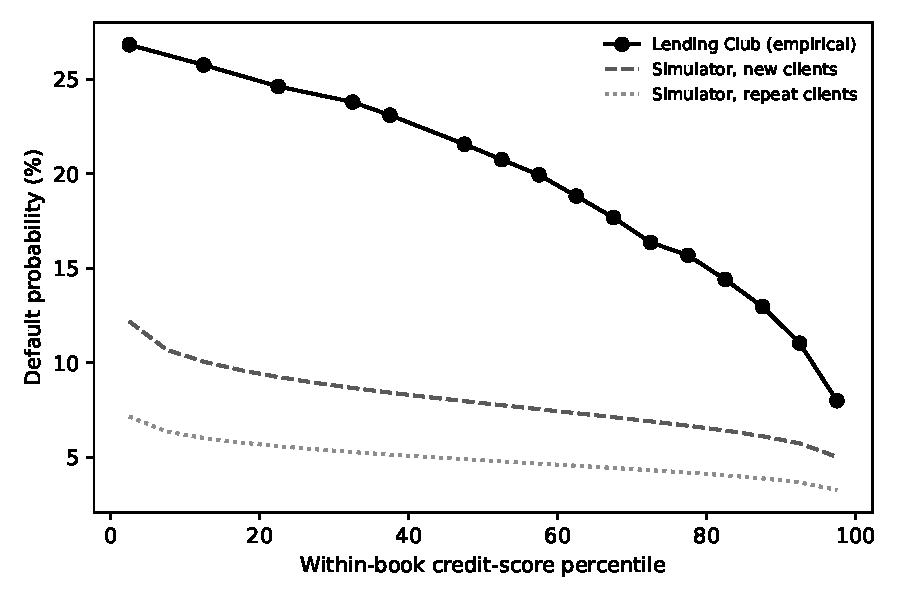
\includegraphics[width=0.72\linewidth]{figures/pd_real_vs_sim.pdf}
    \caption{Default probability by within-book credit-score percentile, simulator curves versus the Lending Club loan book. In Figure~\ref{fig:pd_real_vs_sim}, the within-book percentile axis aligns the two score domains, and the higher Lending Club levels reflect its higher-rate and longer-tenor borrower mix.}
    \label{fig:pd_real_vs_sim}
\end{figure}

\subsection{Why an agent-based simulator}
Loan-level data that jointly record the score, the funding decision, the realised outcome, and the calendar timing across several market regimes are rarely public, because lender underwriting models and outcome histories are proprietary assets \citep{dimaggio2024}. In the absence of such data, an agent-based simulator acts as a controlled laboratory that varies one factor at a time, here the observation dimension, while holding the protocol fixed, which is the comparison that observational data cannot deliver \citep{axtellfarmer2025}. We therefore read the simulator as a tool for studying the structure of the control problem under a fixed training budget, not as a forecast of any single lender's profit.

% ===========================================================================
\section{Conclusion}
% ===========================================================================

This paper evaluates six reinforcement learning algorithms against five rule-based
baselines across six market scenarios and four observation-space sizes (12D, 20D, 30D,
50D) in a controlled credit portfolio simulation, at a training budget of 1{,}500
episodes per seed. The main empirical findings are:

\begin{enumerate}[leftmargin=*,label=(\arabic*)]
    \item The constraint-aware weekly policy remains the best overall controller in every
          dimension by cumulative reward (reward 3{,}666{,}052). On raw realized profit it
          is statistically tied with the profit-oriented policy (3{,}802{,}547 vs.\
          3{,}803{,}168, the latter marginally higher). RL wins zero of six scenarios by
          reward across all dimensions, and zero of six by profit at 20D, 30D, and 50D, but
          two of six at 12D (SAC beats the profit-oriented policy in
          class\_imbalance\_shift and drift, by narrow margins).
    \item The best RL agent is not a single algorithm: SAC leads at 12D (profit
              3{,}785{,}010) and 50D (3{,}724{,}499), A2C at 20D (3{,}761{,}562), and DQN at
          30D (3{,}706{,}594). The profit gap to the best overall controller shrinks to
          between $-$0.46\% (12D) and $-$2.52\% (30D) at every dimension, down from
          $-$9.4\% for the best RL agent (Double-DQN, 12D) under a 30$\times$ smaller
          training budget.
    \item The 30D~to~12D reward improvement for the reference DQN agent is now positive
          \emph{and} statistically significant ($+138{,}516$, $p<10^{-3}$), a reversal from
          the short-budget run, and 30D continues to significantly outperform 50D
          ($+662{,}993$, $p<10^{-3}$), so 30D is the reward-side optimum for this reference
          agent, not only a risk-side compromise.
    \item The best RL agent undercuts the two profit-seeking baselines on default rate in a
          majority of scenarios (5 of 6) at 30D and 50D, but this risk-side advantage is
          weak at 20D (1 of 6) and absent at 12D (0 of 6); the risk-aware weekly policy
          stays the lowest-default controller overall at every dimension. The conditional
          risk-side advantage of RL is therefore dimension-dependent, not universal.
    \item A delayed-evaluation check in the adverse-stress scenario shows DQN statistically
          tied with the static-threshold baseline early in the horizon (week~6, $p=0.345$)
          and significantly ahead by the horizon midpoint (week~25, $+152{,}941$,
          $p<10^{-3}$), a ``locally tied, globally better'' pattern, the opposite of the
          persistent early-and-late deficit found under the short-budget run.
    \item Episode-static behavior, in which threshold volatility is 0.00 throughout the
          episode, is no longer universal: it is specific to the DQN family at 12--30D
          (which only begins adjusting thresholds within the episode at 50D) and to PPO at
          every dimension, while SAC and the actor-critic agents (A2C, A3C) adjust
          thresholds within the episode at every dimension tested.
\end{enumerate}

\noindent
The practical implication has shifted from the short-budget run: training budget, not a
fundamental RL-versus-rule-based ceiling, was the dominant factor behind the earlier
large gap. Well-designed rule-based weekly search still wins the primary reward ranking
in every scenario and dimension tested and needs no training, so it remains the safe
default when training resources are limited, but a sufficiently trained RL agent is now a
credible alternative on profit, and specifically at 30D or 50D it also delivers a real
risk-side (lower default rate) benefit in most scenarios. The 30D observation space is
the strongest default for an RL deployment: it is the only dimension at which the
reference DQN agent's own reward peaks, and it supports the risk-side advantage developed
above. Future work should investigate whether an even larger training budget closes the
remaining $-$0.46\%~to~$-$2.52\% profit gap entirely (particularly for the DQN family at
50D), reward sensitivity to penalty weights, more adaptive recurrent or attention-based
architectures, whether the ``locally tied, globally better'' pattern generalizes beyond
the adverse-stress/30D pairing tested here, and validation on real or semi-synthetic loan
panels.

% ===========================================================================
% REFERENCES  (manual \thebibliography handled by natbib in author-year mode;
% entries are APA-formatted and ordered alphabetically by first author)
% ===========================================================================
\begin{thebibliography}{Zhang and Yu(2023)}

    \bibitem[Arulkumaran et~al.(2017)]{arulkumaran2017}
    Arulkumaran, K., Deisenroth, M.~P., Brundage, M., \& Bharath, A.~A. (2017).
    Deep reinforcement learning: A brief survey.
    \textit{IEEE Signal Processing Magazine, 34}(6), 26--38.
    \url{https://doi.org/10.1109/MSP.2017.2743240}

    \bibitem[Axtell \& Farmer(2025)]{axtellfarmer2025}
    Axtell, R.~L., \& Farmer, J.~D. (2025).
    Agent-based modeling in economics and finance: Past, present, and future.
    \textit{Journal of Economic Literature}.
    \url{https://doi.org/10.1257/jel.20221319} % TODO add volume/issue/pages once assigned

    \bibitem[Baesens et~al.(2003)]{baesens2003}
    Baesens, B., Van Gestel, T., Viaene, S., Stepanova, M., Suykens, J., \& Vanthienen, J. (2003).
    Benchmarking state-of-the-art classification algorithms for credit scoring.
    \textit{Journal of the Operational Research Society, 54}(6), 627--635.
    \url{https://doi.org/10.1057/palgrave.jors.2601545}

    \bibitem[Bank of Russia(2025)]{cbr2025}
    Bank of Russia. (2025).
    \textit{Financial stability review}. Bank of Russia.
    \url{https://www.cbr.ru/eng/analytics/finstab/ofs/} % TODO confirm exact issue and reporting period

    \bibitem[Bellotti \& Crook(2009)]{bellotti2009}
    Bellotti, T., \& Crook, J. (2009).
    Support vector machines for credit scoring and discovery of significant features.
    \textit{Expert Systems with Applications, 36}(2), 3302--3308.
    \url{https://doi.org/10.1016/j.eswa.2008.01.005}

    \bibitem[Brown \& Mues(2012)]{brownmues2012}
    Brown, I., \& Mues, C. (2012).
    An experimental comparison of classification algorithms for imbalanced credit scoring data sets.
    \textit{Expert Systems with Applications, 39}(3), 3446--3453.
    \url{https://doi.org/10.1016/j.eswa.2011.09.033}

    \bibitem[Dayan \& Niv(2008)]{dayan2008}
    Dayan, P., \& Niv, Y. (2008).
    Reinforcement learning: The good, the bad and the ugly.
    \textit{Current Opinion in Neurobiology, 18}(2), 185--196.
    \url{https://doi.org/10.1016/j.conb.2008.08.003}

    \bibitem[Di Maggio et~al.(2024)]{dimaggio2024}
    Di Maggio, M., Ratnadiwakara, D., \& Carmichael, D. (2024).
    Invisible primes: Fintech lending with alternative data.
    \textit{Management Science}.
    \url{https://doi.org/10.1287/mnsc.2024.07854} % TODO add volume/issue/pages once assigned

    \bibitem[Gunnarsson et~al.(2021)]{gunnarsson2021}
    Gunnarsson, B.~R., vanden Broucke, S., Baesens, B., \'Oskarsd\'ottir, M., \& Lemahieu, W. (2021).
    Deep learning for credit scoring: Do or don't?
    \textit{European Journal of Operational Research, 295}(1), 292--305.
    \url{https://doi.org/10.1016/j.ejor.2021.03.006}

    \bibitem[Haarnoja et~al.(2018)]{haarnoja2018sac}
    Haarnoja, T., Zhou, A., Abbeel, P., \& Levine, S. (2018).
    Soft actor-critic: Off-policy maximum entropy deep reinforcement learning with a
    stochastic actor. In \textit{Proceedings of the 35th International Conference on Machine
        Learning} (PMLR 80, pp.~1861--1870).
    \url{https://proceedings.mlr.press/v80/haarnoja18b.html}

    \bibitem[Hand \& Henley(1997)]{hand1997}
    Hand, D.~J., \& Henley, W.~E. (1997).
    Statistical classification methods in consumer credit scoring: A review.
    \textit{Journal of the Royal Statistical Society: Series A, 160}(3), 523--541.
    \url{https://doi.org/10.1111/j.1467-985X.1997.00078.x}

    \bibitem[Herasymovych et~al.(2019)]{herasymovych2019}
    Herasymovych, M., M\"arka, K., \& Lukason, O. (2019).
    Using reinforcement learning to optimize the acceptance threshold of a credit scoring model.
    \textit{Applied Soft Computing, 84,} 105697.
    \url{https://doi.org/10.1016/j.asoc.2019.105697}

    \bibitem[Kiatsupaibul et~al.(2024)]{kiatsupaibul2024}
    Kiatsupaibul, S., Chansiripas, P., Manopanjasiri, P., Visantavarakul, K., \& Wen, Z. (2024).
    \textit{Reinforcement learning in credit scoring and underwriting} [Preprint]. arXiv.
    \url{https://doi.org/10.48550/arXiv.2212.07632}

    \bibitem[Lessmann et~al.(2015)]{lessmann2015}
    Lessmann, S., Baesens, B., Seow, H.-V., \& Thomas, L.~C. (2015).
    Benchmarking state-of-the-art classification algorithms for credit scoring: An update of research.
    \textit{European Journal of Operational Research, 247}(1), 124--136.
    \url{https://doi.org/10.1016/j.ejor.2015.05.030}

    \bibitem[Loterman et~al.(2012)]{loterman2012}
    Loterman, G., Brown, I., Martens, D., Mues, C., \& Baesens, B. (2012).
    Benchmarking regression algorithms for loss given default modeling.
    \textit{International Journal of Forecasting, 28}(1), 161--170.
    \url{https://doi.org/10.1016/j.ijforecast.2011.01.006}

    \bibitem[Nallakaruppan et~al.(2024)]{nallakaruppan2024}
    Nallakaruppan, M.~K., Balusamy, B., Shri, M.~L., Malathi, V., \& Bhattacharyya, S. (2024).
    An explainable AI framework for credit evaluation and analysis.
    \textit{Applied Soft Computing, 153,} 111307.
    \url{https://doi.org/10.1016/j.asoc.2024.111307}

    \bibitem[Qi \& Zhao(2011)]{qi2011}
    Qi, M., \& Zhao, X. (2011).
    Comparison of modeling methods for loss given default.
    \textit{Journal of Banking \& Finance, 35}(11), 2842--2855.
    \url{https://doi.org/10.1016/j.jbankfin.2011.03.011}

    \bibitem[Raffin et~al.(2021)]{stable_baselines3}
    Raffin, A., Hill, A., Gleave, A., Kanervisto, A., Ernestus, M., \& Dormann, N. (2021).
    Stable-Baselines3: Reliable reinforcement learning implementations.
    \textit{Journal of Machine Learning Research, 22}(268), 1--8.
    \url{http://jmlr.org/papers/v22/20-1364.html}

    \bibitem[Schulman et~al.(2017)]{schulman2017ppo}
    Schulman, J., Wolski, F., Dhariwal, P., Radford, A., \& Klimov, O. (2017).
    \textit{Proximal policy optimization algorithms} [Preprint]. arXiv.
    \url{https://doi.org/10.48550/arXiv.1707.06347}

    \bibitem[Siddiqi(2006)]{siddiqi2006}
    Siddiqi, N. (2006).
    \textit{Credit risk scorecards: Developing and implementing intelligent credit scoring}. Wiley.

    \bibitem[Thomas(2017)]{thomas2017}
    Thomas, L.~C. (2017).
    \textit{Credit scoring and its applications} (2nd ed.).
    Society for Industrial and Applied Mathematics.
    \url{https://doi.org/10.1137/1.9781611974560}

    \bibitem[van Hasselt et~al.(2016)]{van2016ddqn}
    van Hasselt, H., Guez, A., \& Silver, D. (2016).
    Deep reinforcement learning with double Q-learning. In \textit{Proceedings of the 30th
        AAAI Conference on Artificial Intelligence} (Vol.~30, pp.~2094--2100). AAAI Press.
    \url{https://doi.org/10.1609/aaai.v30i1.10295}

    \bibitem[Xia et~al.(2017)]{xia2017}
    Xia, Y., Liu, C., Li, Y., \& Liu, N. (2017).
    A boosted decision tree approach using Bayesian hyper-parameter optimization for credit scoring.
    \textit{Expert Systems with Applications, 78,} 225--241.
    \url{https://doi.org/10.1016/j.eswa.2017.02.017}

    \bibitem[Yang et~al.(2024)]{yang2024}
    Yang, D., Xiao, B., Cao, M., \& Shen, H. (2024).
    A new hybrid credit scoring ensemble model with feature enhancement and soft voting weight optimization.
    \textit{Expert Systems with Applications, 238,} 122101.
    \url{https://doi.org/10.1016/j.eswa.2023.122101}

    \bibitem[Zhang \& Yu(2023)]{zhangyu2023}
    Zhang, X., \& Yu, L. (2023).
    Consumer credit risk assessment: A review from the state-of-the-art classification
    algorithms, data traits, and learning methods.
    \textit{Expert Systems with Applications, 237,} 121484.
    \url{https://doi.org/10.1016/j.eswa.2023.121484}

\end{thebibliography}

% ===========================================================================
\appendix
% ===========================================================================

\section{Simulator details}
\label{app:simulator}

This appendix specifies the data-generating process so that the experiments can be reproduced from the public repository. All values are the calibrated full-profile settings.

\paragraph{Applicant generation.}
Each interactive week the simulator draws a base application volume around 600 applications, scales it by a seasonal factor and multiplicative volume noise, and splits it into new and repeat counts through two Poisson draws. The repeat share follows a scenario base level modulated by an annual seasonal term and clamped to $[0.15, 0.75]$. Each applicant in segment $s$ receives a credit score drawn from a Gaussian $\mathcal{N}(\mu_s, \sigma_s)$ clipped to $[0,100]$, with $\mu_{\text{new}}=59$, $\sigma_{\text{new}}=13$ and $\mu_{\text{repeat}}=69$, $\sigma_{\text{repeat}}=10$ in the base market.

\paragraph{Default and recovery.}
An applicant with score $x$ in segment $s$ defaults with probability
\begin{equation}
    p_s(x) = \sigma\!\left(\beta_s - \kappa_s \cdot \tfrac{x-50}{10}\right),
    \label{eq:pd}
\end{equation}
clipped to $[0.01, 0.98]$, where $\sigma$ is the logistic function and $\beta_{\text{new}}=-2.3$, $\kappa_{\text{new}}=0.18$, $\beta_{\text{repeat}}=-2.6$, $\kappa_{\text{repeat}}=0.20$ in the base market. Scenario stress shifts $\beta_s$ gradually over the horizon and an abrupt shock adds to $\beta_s$ from the shock week onward (Table~\ref{tab:scenario_params}). These settings target portfolio default rates of 4--6\% in the base market and 9--14\% under adverse stress. A defaulted loan recovers with probability $r_{\text{new}}=0.26$ or $r_{\text{repeat}}=0.34$, and on recovery the lender receives the principal plus a fraction $\varphi_s$ of the scheduled interest, with $\varphi_{\text{new}}=0.65$ and $\varphi_{\text{repeat}}=0.72$.

\paragraph{Loan terms and cashflows.}
The principal is lognormal with mean $A_{\text{new}}=1650$ or $A_{\text{repeat}}=2150$ currency units and log-scale $0.28$ (new) or $0.25$ (repeat), clipped to $[300, 9000]$ and scaled by the scenario loan-amount multiplier. Each loan receives an integer term $d$ in months (new: 5--12, repeat: 4--10) and a scheduled interest income of $\text{principal}\times(\rho_s\, d/12 + o_s)$, with annual fee rate $\rho_{\text{new}}=0.16$, $\rho_{\text{repeat}}=0.13$ and origination $o_{\text{new}}=0.035$, $o_{\text{repeat}}=0.03$. Outcomes enter a forward event queue: a repaid loan returns the interest at week $\text{issue}+d$, a defaulted loan returns $-\text{principal}$ at week $\text{issue}+d$, and a recovered loan adds the recovery value a further 1--4 weeks later. The term index $d$ therefore sets both the interest horizon $d/12$ years and the event delay $d$ weeks. Each cashflow is discounted to net present value at a weekly rate of $0.14/52$, that is an annual discount rate of 14\%.

\paragraph{Episode structure and capital.}
Each episode runs an 8-week warm-up at the default thresholds (60 for new, 50 for repeat), then a 52-week interactive horizon, then a terminal settlement that resolves all pending events so that loans originated near the horizon are not penalised. Outstanding principal plus the principal accepted in the current week is tracked against a capital limit of 3{,}000{,}000 to form the capital-usage ratio used in the reward.

\begin{table}[H]
    \centering
    \footnotesize
    \caption{Per-scenario stress parameters. In Table~\ref{tab:scenario_params}, the score and default shifts are total drifts applied gradually over the horizon, and the shock column gives the magnitude added to the default intercept and the week it begins.}
    \label{tab:scenario_params}
    \resizebox{\linewidth}{!}{%
        \begin{tabular}{l c c c c c c}
            \toprule
            Scenario                & Repeat share & Score shift (new/rep) & Default shift (new/rep) & Score noise & Loan mult. & Shock (week) \\
            \midrule
            base\_market            & 0.35         & $0.00$ / $0.00$       & $0.00$ / $0.00$         & 1.00        & 1.00       & none         \\
            drift                   & 0.34         & $-0.18$ / $-0.07$     & $0.18$ / $0.08$         & 1.00        & 1.00       & 0.08 (13)    \\
            adverse\_stress         & 0.33         & $-0.10$ / $-0.10$     & $0.30$ / $0.22$         & 1.15        & 1.15       & 0.22 (10)    \\
            class\_imbalance\_shift & 0.28         & $-0.08$ / $0.03$      & $0.12$ / $-0.02$        & 1.00        & 0.95       & 0.12 (16)    \\
            noise                   & 0.35         & $0.00$ / $0.00$       & $0.04$ / $0.04$         & 1.45        & 1.00       & none         \\
            split\_policy\_dynamics & 0.38         & $-0.20$ / $0.10$      & $0.22$ / $-0.10$        & 1.00        & 1.00       & 0.06 (14)    \\
            \bottomrule
        \end{tabular}}
\end{table}

\section{Training hyperparameters}
\label{app:hyperparams}

In Table~\ref{tab:hyperparams}, the shared training configuration for the full-profile
run is listed. The settings are held identical across all four state sizes, so any
performance difference between dimensions is attributable to the observation vector
rather than to the training recipe.

\begin{table}[H]
    \centering
    \small
    \caption{Shared training settings (full-profile run), held identical across all four state sizes. In Table~\ref{tab:hyperparams}, these settings are fixed so that any difference across dimensions reflects the observation vector rather than the training recipe.}
    \label{tab:hyperparams}
    \begin{tabular}{l l l}
        \toprule
        Parameter                & Value                           & Notes                      \\
        \midrule
        Network architecture     & MLP, $2\times 128$ hidden units & Shared across all agents   \\
        Discount factor $\gamma$ & $0.98$                          & Standard                   \\
        Learning rate            & SB3 default (varies by agent)   & Not tuned                  \\
        Training episodes/seed   & 1{,}500                         & Full profile               \\
        Seeds                    & 11, 23, 37, 51, 67, 79, 97, 113 & 8 seeds, fixed across dims \\
        Evaluation runs          & 12 per seed per scenario        & Same protocol across dims  \\
        Threshold grid           & $[35, 85]$ in steps of 5        & 11 actions per segment     \\
        Warm-up weeks            & 8                               & Pre-fills loan book        \\
        Interactive horizon      & 52 weeks                        & Full profile               \\
        Applications per week    & 600                             & Before scale factors       \\
        Bootstrap resamples      & 1000                            & 95\% CI                    \\
        \bottomrule
    \end{tabular}
\end{table}

\begin{table}[H]
    \centering
    \small
    \caption{Per-agent reinforcement-learning hyperparameters (full-profile run), held identical across all four state sizes. In Table~\ref{tab:agent_hyperparams}, A2C, PPO, and SAC use Stable-Baselines3 \citep{stable_baselines3}, while DQN, Double-DQN, and A3C use matched custom PyTorch implementations.}
    \label{tab:agent_hyperparams}
    \begin{tabular}{l l p{0.5\linewidth}}
        \toprule
        Agent      & Implementation & Key hyperparameters                                                                                                                                                          \\
        \midrule
        DQN        & Custom         & lr $10^{-3}$, batch 64, replay $2\times10^{4}$, learning starts 300, train freq 1, gradient steps 1, target update 200, $\varepsilon$ $1.0\!\to\!0.05$ over 65\% of training \\
        Double-DQN & Custom         & As DQN, with a double-Q target                                                                                                                                               \\
        PPO        & SB3            & lr $3\times10^{-4}$, rollout $n=256$, batch 64, GAE $\lambda$ 0.95, entropy coef 0.01, clip range 0.20                                                                       \\
        A2C        & SB3            & lr $7\times10^{-4}$, rollout $n=256$, GAE $\lambda$ 0.95, entropy coef 0.01                                                                                                  \\
        A3C        & Custom         & lr $5\times10^{-4}$, entropy coef 0.01, value coef 0.5, full-episode rollouts (single worker)                                                                                \\
        SAC        & SB3            & lr $3\times10^{-4}$, buffer $5\times10^{4}$, learning starts 500, batch 128, $\tau$ 0.02, train freq 1, gradient steps 1                                                     \\
        \bottomrule
    \end{tabular}
\end{table}

% ===========================================================================
% ELSEVIER FORMALITIES
% ===========================================================================

\section*{CRediT authorship contribution statement}

\textbf{Evgeny Baulin:} Software, Investigation, Writing -- original draft.
\textbf{P.~P.~Lukianchenko:} Supervision, Writing -- review \& editing.

\section*{Declaration of competing interest}

The authors declare that they have no known competing financial interests or personal
relationships that could have appeared to influence the work reported in this paper.

\section*{Acknowledgements}

This work was supported by the Ministry of Economic Development of the Russian
Federation under Agreement 139-15-2025-011 (identifier 000000C313925P4G0002).
\end{document}
